% begin module tangents-reminder
\begin{frame}
\frametitle{Tangents}
\begin{center}
\psset{xunit=0.8cm, yunit=0.8cm}
\begin{pspicture}(-2.7, -0.7)(2.7,6.4)
\tiny
\fcLabelXOne
\fcLabelYOne
\rput[l](0.2, 3.5){$y=x^2$}
\psaxes[ticks=none, labels=none]{<->}(0,0)(-1,-0.5)(2.5,4.5)
%Function formula: (x)^{2}
\psplot[linecolor=red, plotpoints=1000]{-1}{2.5}{x 2 exp }
\psline[linecolor=blue](0.25, -0.5)(2.5,4)
\fcFullDot{1}{1}
\rput[lt](1.1, 0.9){$P=(1,1)$}
\end{pspicture}
%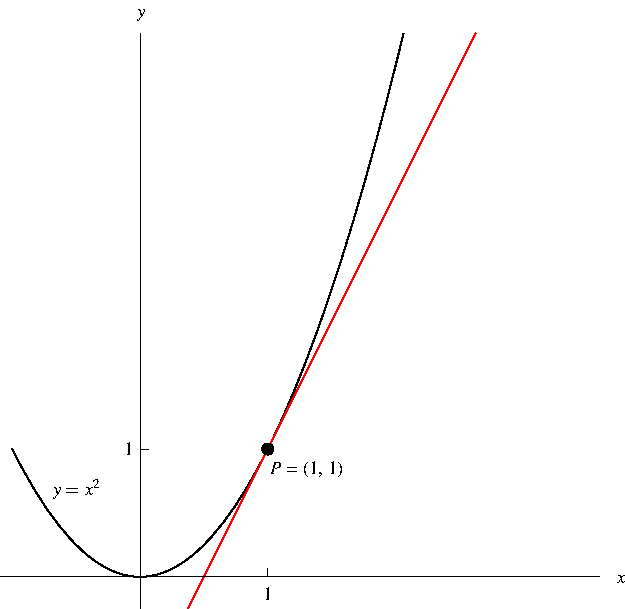
\includegraphics[height=5cm]{derivatives/pictures/02-01-secanta.pdf}%
\end{center}
\begin{itemize}
\item<2->  Recall that in preceding lectures we tried to find the tangent line to the curve $y = x^2$ at the point $P = (1,1)$.
\item<3->  This problem motivated us to study limits.
\end{itemize}
\end{frame}


\begin{frame}
\begin{columns}[c]
\column{.45\textwidth}
\psset{xunit=0.8cm, yunit=0.8cm}
\begin{pspicture}(-1,-1.5)(5.4,4.6)
\psaxes[ticks=none, labels=none]{<->}(0,0)(-1,-1.5)(5.4,4.6)
%Function formula: -11/8+5/18 ((x) ((x) (x)))-1/81 ((x) ((x) ((x) (x))))-73/36 ((x) (x))+43/8 (x)
\psplot[linecolor=red, plotpoints=1000]{0}{5}{x 5.375 mul x x mul -2.02778 mul add x x mul x mul x mul -0.0123457 mul add x x mul x mul 0.277778 mul add -1.375 add }

\uncover<1,11->{
\psline[linecolor=blue](0, -0.935185185)(1.531304348, 4.5)
\fcFullDot{0.5}{0.839506173}
}

\rput[rb] (0.6,0.92){\tiny$P=(a, f(a))$}
\rput[t](0.5, -0.1){\tiny$a$}
\psline(0.5,0.1)(0.5,0)
\uncover<handout:0|2-10>{
\psline[linestyle=dashed](0.5, 0)(0.5, 0.839506173)
}

\uncover<handout:0|10>{
\psline[linecolor=blue](0, -0.558641975)(1.809050773, 4.5)
\fcFullDot{1}{2.237654321}
\psline[linestyle=dashed](1, 0)(1, 2.237654321)
\psline(0.5, 0.839506173)(1,0.839506173) (1, 2.237654321)
\rput[t](1, -0.1){\tiny$x$}
\rput[l](1.1, 1.5){\tiny$f(x)-f(a)$}
\rput[t](0.75, 0.82){\tiny$x-a$}
\rput[b](1, 4){\tiny $Q=(x,f(x))$}
\psline[linestyle=dotted]{->}(1,3.9)(1, 2.237654321)
}

\uncover<handout:1|9>{
\psline[linecolor=blue](0, -0.240741)(2.19429, 4.5)
\fcFullDot{1.5}{3}
\psline[linestyle=dashed](1.5, 0)(1.5, 3)
\psline(0.5, 0.839506173)(1.5,0.839506173) (1.5, 3)
\rput[t](1.5, -0.1){\tiny$x$}
\rput[l](1.6, 1.9){\tiny$f(x)-f(a)$}
\rput[t](1, 0.82){\tiny$x-a$}
\rput[b](1.5, 4){\tiny $Q=(x,f(x))$}
\psline[linestyle=dotted]{->}(1.5,3.9)(1.5, 3)
}

\uncover<handout:0|8>{
\psline[linecolor=blue](0, 0.0231481)(2.74197, 4.5)
\fcFullDot{2}{3.28858}
\psline[linestyle=dashed](2, 0)(2, 3.28858)
\psline(0.5, 0.82)(2,0.839506173) (2, 3.28858)
\rput[t](2, -0.1){\tiny$x$}
\rput[l](2.1, 2){\tiny$f(x)-f(a)$}
\rput[t](1.25, 0.82){\tiny$x-a$}
\rput[b](2, 4){\tiny $Q=(x,f(x))$}
\psline[linestyle=dotted]{->}(2,3.9)(2, 3.28858)
}

\uncover<handout:0|7>{
\psline[linecolor=blue](0, 0.237654)(3.54103, 4.5)
\fcFullDot{2.5}{3.24691}
\psline[linestyle=dashed](2.5, 0)(2.5, 3.24691)
\psline(0.5, 0.839506173)(2.5,0.839506173) (2.5, 3.24691)
\rput[t](2.5, -0.1){\tiny$x$}
\rput[l](2.6, 2){\tiny$f(x)-f(a)$}
\rput[t](1.5, 0.82){\tiny$x-a$}
\rput[b](2.5, 4){\tiny $Q=(x,f(x))$}
\psline[linestyle=dotted]{->}(2.5,3.9)(2.5, 3.24691)
}

\uncover<handout:0|6>{
\psline[linecolor=blue](0, 0.407407)(4.73571, 4.5)
\fcFullDot{3}{3}
\psline[linestyle=dashed](3, 0)(3, 3)
\psline(0.5, 0.839506173)(3,0.839506173) (3, 3)
\rput[t](3, -0.1){\tiny$x$}
\rput[l](3.1, 1.9){\tiny$f(x)-f(a)$}
\rput[t](1.75, 0.82){\tiny$x-a$}
\rput[b](3, 4){\tiny $Q=(x,f(x))$}
\psline[linestyle=dotted]{->}(3,3.9)(3, 3)
}

\uncover<handout:0|5>{
\psline[linecolor=blue](0, 0.537037)(5, 3.56173)
\fcFullDot{3.5}{2.65432}
\psline[linestyle=dashed](3.5, 0)(3.5, 2.65432)
\psline(0.5, 0.839506173)(3.5,0.839506173) (3.5, 2.65432)
\rput[t](3.5, -0.1){\tiny$x$}
\rput[l](3.6, 1.7){\tiny$f(x)-f(a)$}
\rput[t](2, 0.82){\tiny$x-a$}
\rput[b](3.5, 4){\tiny $Q=(x,f(x))$}
\psline[linestyle=dotted]{->}(3.5,3.9)(3.5, 2.65432)
}

\uncover<handout:0|2-4>{
\psline[linecolor=blue](0, 0.631173)(5, 2.71451)
\fcFullDot{4}{2.29784}
\psline[linestyle=dashed](4, 0)(4, 2.29784)
\psline(0.5, 0.839506173)(4,0.839506173) (4, 2.29784)
\rput[t](4, -0.1){\tiny$x$}
\rput[l](4.1, 1.5){\tiny$f(x)-f(a)$}
\rput[t](2.25, 0.82){\tiny$x-a$}
\rput[b](4, 4){\tiny $Q=(x,f(x))$}
\psline[linestyle=dotted]{->}(4,3.9)(4, 2.29784)
}
\end{pspicture}
%\ \only<handout:0| -1,11->{%
%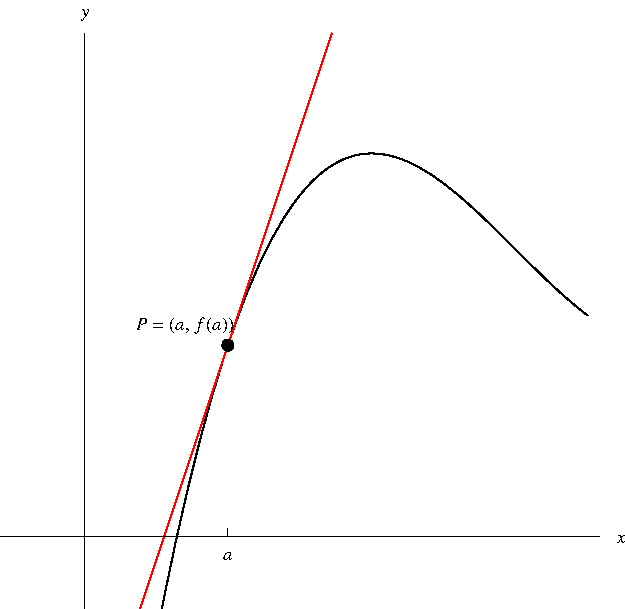
\includegraphics[height=4.5cm]{derivatives/pictures/03-01-tangent.pdf}%
%}%
%\only<2-4>{%
%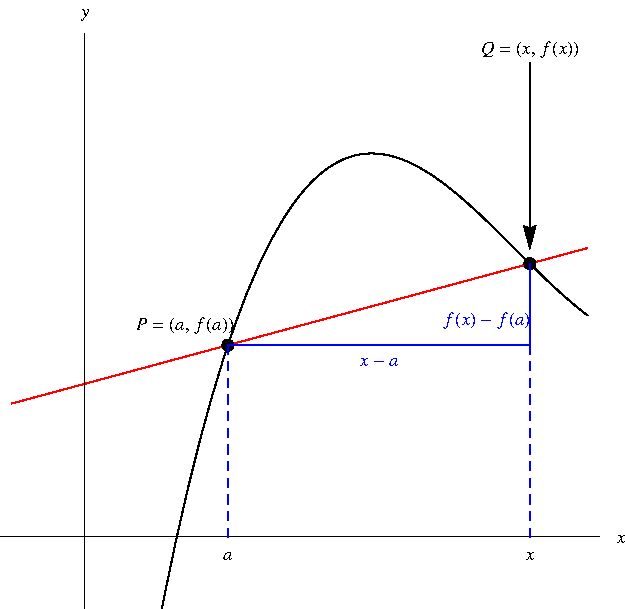
\includegraphics[height=4.5cm]{derivatives/pictures/03-01-secanta.pdf}%
%}%
%\only<handout:0| 5>{%
%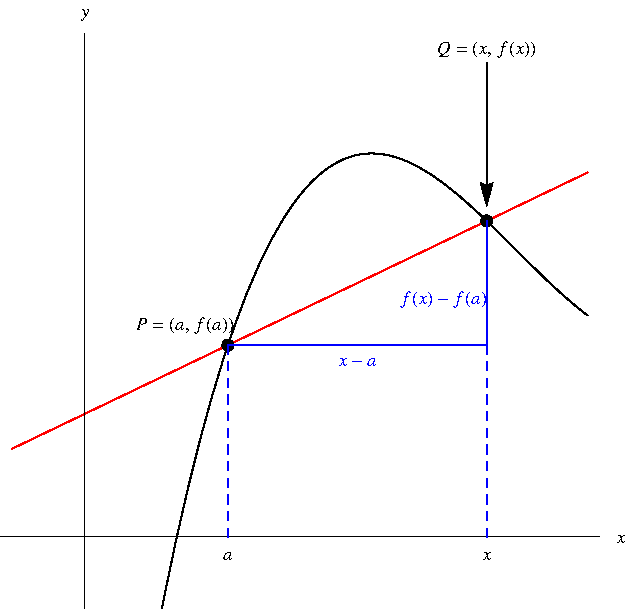
\includegraphics[height=4.5cm]{derivatives/pictures/03-01-secantb.pdf}%
%}%
%\only<handout:0| 6>{%
%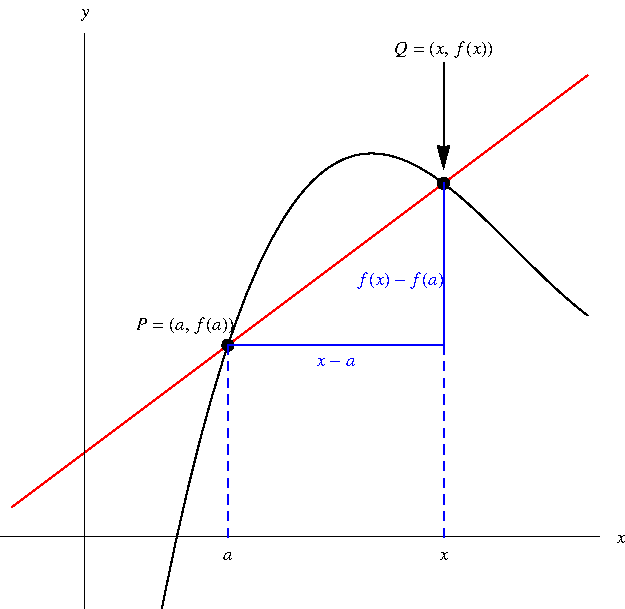
\includegraphics[height=4.5cm]{derivatives/pictures/03-01-secantc.pdf}%
%}%
%\only<handout:0| 7>{%
%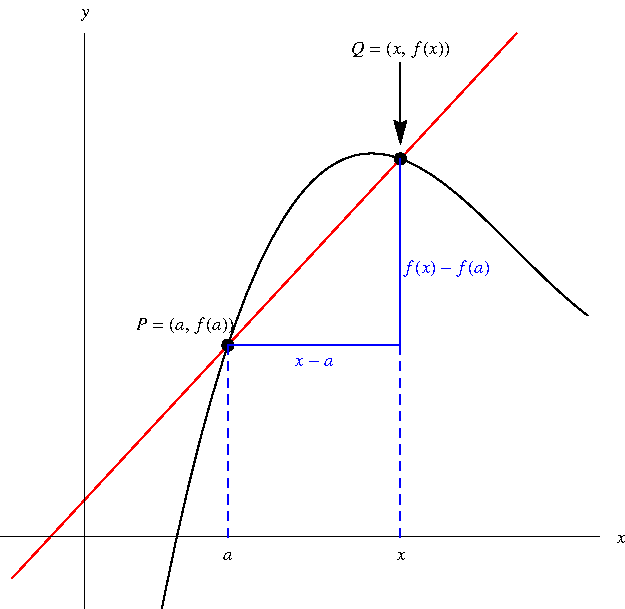
\includegraphics[height=4.5cm]{derivatives/pictures/03-01-secantd.pdf}%
%}%
%\only<handout:0| 8>{%
%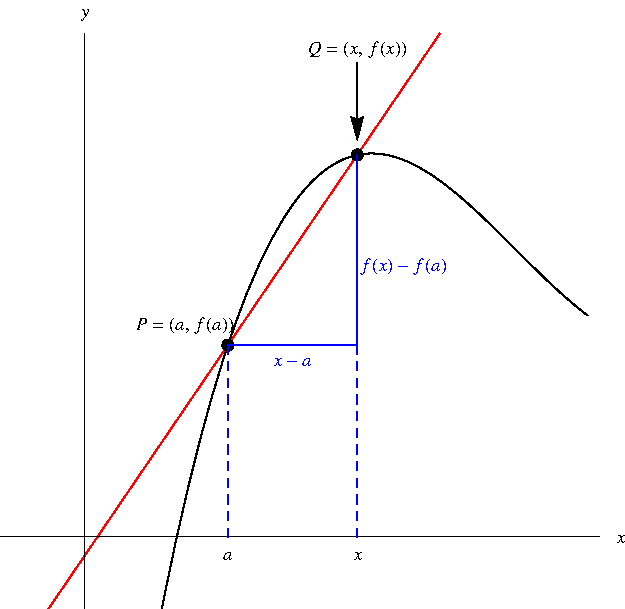
\includegraphics[height=4.5cm]{derivatives/pictures/03-01-secante.pdf}%
%}%
%\only<handout:0| 9>{%
%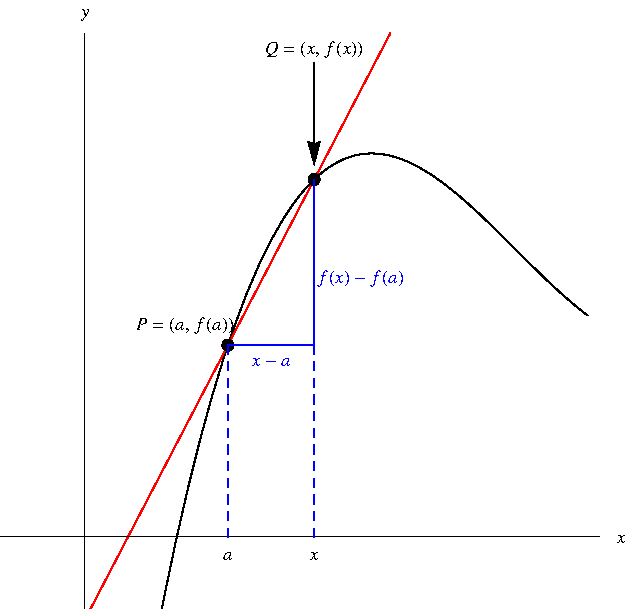
\includegraphics[height=4.5cm]{derivatives/pictures/03-01-secantf.pdf}%
%}%
%\only<handout:0| 10>{%
%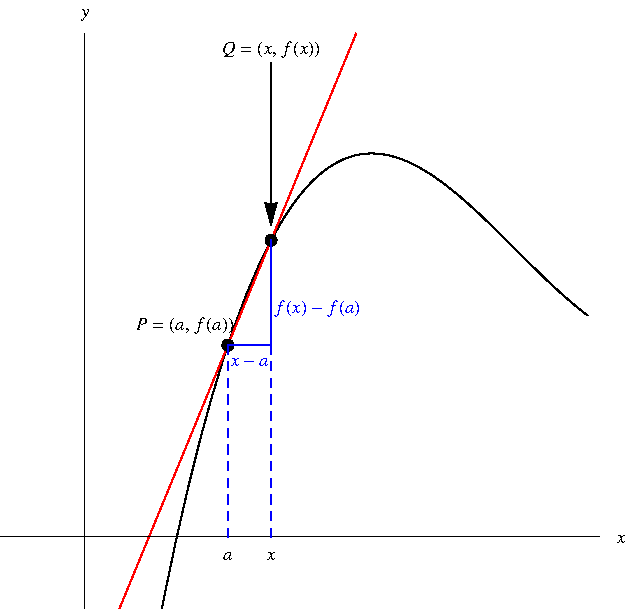
\includegraphics[height=4.5cm]{derivatives/pictures/03-01-secantg.pdf}%
%}%

\column{.55\textwidth}
\begin{itemize}
\item<1->  How to find the tangent line to the curve $y = f(x)$ at $P = (a, f(a))$?
\item<2->  Consider nearby point $Q = (x, f(x))$.
\item<3->  Compute slope of secant line $PQ$: $m_{PQ} = \frac{f(x)-f(a)}{x-a}$.
\item<4->  As $x$ approaches $a$, the point $Q$ approaches $P$.
\end{itemize}
\end{columns}
\uncover<11->{%
\small
\begin{definition}[Non-vertical tangent line]
Let $P = (a, f(a))$. Suppose the limit $\displaystyle m=\lim_{x\rightarrow a}\frac{f(x) - f(a)}{x-a}$
exists. Define the \alertNoH{11}{tangent to $y=f(x)$ at $P$} to be \alertNoH{12}{the line passing through $P$ with slope $m$}\uncover<12->{, in other words, \alertNoH{12}{the line with equation}} \uncover<13->{$\alertNoH{13}{y-f(a)=m(x-a) }$.}
\end{definition}
\uncover<14>{
\textbf{Note. } Even if the limit does not exist a reasonable notion of a tangent line may still exist.
}
}%
\end{frame}
% end module tangents-reminder
